%!TEX root = main.tex
\section{User Study Evaluation}
\subsection{Procedure}
Given that our preliminary study motivated our desiderata for the metrics and constraints used in the problem formulation, we further evaluate the utility of our tool by performing a user study focusing on addressing the research questions: 
\begin{itemize}
	\item RQ1: How effective is our tool at summarizing key insights within a given dataset?
	\item RQ2: How effective is our tool in providing analysts with task-specific insights? (including understanding causal explanations, identification of interesting visualization, and finding outliers[?])
	\item RQ3: How useful are the visualizations in the recommended dashboard to analysts?
\end{itemize}
\par We recruited 18 participants who have prior experience working with data. This can include, but are not limited to, browsing and reading data, data cleaning and wrangling, data visualization and model building. The inclusion criteria is assessed based on a self-reporting basis in the pre-study survey. Figure --- shows the demographics of participants. None of the participants have prior experience in working with the two datasets used in the study.
\par In this between-group study, participants are randomly assigned two of the three conditions. 
\begin{enumerate}
	\item \system: Dashboard picked by the frontier greedy algorithm, as described in Section \ref{algorithms}. The chosen visualizations are displayed in a graph layout.
	\item Clustering (\textit{Cluster}): K-Means clustering is performed on the dataset with k clusters. For each representative cluster, pick the visualization that is closest to the cluster center and display the visualization in table layout in the order of increasing number of conditions in the filter combination. The chosen visualizations are displayed in a 5x2 table layout.
	% \item Parent-Child Pairs (\textit{PC}) : Pick top k/2 parent-child pairs without enforcing informative criterion. Display as pairs of disconnected graph.
	\item Levelwise BFS (\textit{BFS}) : k visualizations is selected in level-wise order and displayed in a graph layout. This baseline is designed to simulate the scroll-browsing behavior of a visualization dashboard. The chosen visualizations are displayed in a 5x2 table layout.
	% \item Random (\textit{Rand}) [OPTIONAL]: k visualizations is randomly selected and display in table layout. This is intended to simulate user behavior on free-form visualization generation tool, where users add arbitrary combinations of filters to explore an unfamiliar dataset.
	%\item Direct manipulation: Allow users to add arbitrary combinations of filters and facets. Record insights until k visualizations seen. Display in table layout.
	%\item Direct manipulation (\textit{DM}): Through expert crowdsourcing, we asked a group of expert users to add arbitrary combinations of filters and facets to create a dashboard of k visualization while given a time constraint of 30 minutes. These expert-generated dashboards are used as the DM baselines viewed by all other users in the user study. \footnote{We chose not to perform a comparison with a Tableau-like interface, since activities involved in free-form DM and our tool is fundamentally different. Direct manipulation engages users in the act of visualization construction and browsing through an iterative workflow, while our displayed dashboard only require the users to browse a set of recommendation. The confounding variable related to the cost-benefit tradeoff between visualization construction versus browsing is an unaddressed but interesting direction of research for visualization recommendation.}
\end{enumerate}
All generated dashboards had k=10 visualizations. We ensure that the ordering for each combination is randomized to prevent confounding learning effects. 
\par The study begins with a 5 minute tutorial using dashboards generated for the Titanic dataset. To prevent participant's bias, participants were not provided an explanation of how the dashboard is generated and why the visualizations were arranged in a particular way. Then, participants proceeded onto the Police dataset\footnote{\url{https://openpolicing.stanford.edu/data/}} %, which contains visualizations of the \% of police stop that resulted in a warning, ticket, or an arrest.
, which contains a total of 312948 records of vehicle and pedestrian stops from law enforcement departments in Connecticut, dated from 2013 to 2015. We generate a dashboard of visualizations based on whether the police stop resulted in the driver getting a ticket, warning, or arrest/summons. The attributes in the dataset include driver gender, age, race, and the stop time of day, whether a search was conducted, and whether contraband was found.

\par Participants were given some time to read through a worksheet containing descriptions of the data attributes. Participants were given an attention check question where they are asked to find and read off the values of a visualization in the dashboard. In the main experiment, participants were asked to accomplish the following tasks in the prescribed order below:
\par \textbf{Retrieval:} Participants were asked to talk aloud as they interpret the visualizations in the dashboard and mark each visualization as either interesting, not interesting or unselected.
\par \textbf{Attribute Ranking:} Participants were given a worksheet with all the attributes listed and asked to rank the variable in order of importance in contributing to one particular x-axis value (e.g. stop outcome = arrest)
\par \textbf{Shallow Prediction:} Participants were given a separate worksheet and asked to draw an estimate of the visualization of an unseen visualization. The visualization to be estimated is ``shallow'' in the sense that it is a 2-combination filter, with one parent in the given dashboard. After making the prediction, participants are shown the value of the actual data distribution and asked to rate on a Likert scale of 10 how surprising was the result.
\par \textbf{Deep Prediction:} Similar to the shallow prediction, except the visualization to be estimated is ``deep'' in the sense that it is a 3-combination filter, with only one parent in the given dashboard. 
\par The second dataset in the study is the Autism dataset\footnote{\url{https://archive.ics.uci.edu/ml/datasets/Autism+Screening+Adult}}, which includes the result of autism spectrum disorder screening for 704 adults. The attributes in the dataset are  binary responses to 10 questions that are part of the screening process. Participants are not given the descriptions of the questions nor the answers corresponding to the labels. We generate dashboard visualizations based on whether the participant is diagnosed with autism or not. We repeat the same procedure described above for the Autism dataset. At the end of the study, we asked two open-ended questions regarding the stories and insights that they have learned and what they liked or didn't liked about each dashboard.
%The user study is composed of two phases. Phase one of the experiment focuses on comparing our tool against a set of baselines intended to simulate the natural sequence of visualizations that an analyst would encounter through various approaches during exploratory analysis. The baselines include: 
%To prevent learning effects, the ordering of the baselines will be randomized across users. 
% \par At the beginning of the study, participants were provided with a dashboard from an example dataset, as well as an explanation of how the dashboard is generated. For each of the visualization dashboard, participants are asked to mark visualizations as interesting/not interesting while explaining their reasoning for each annotation. Then, they are asked to summarize a list of insights that they have discovered after browsing through all visualizations in the dashboard. Participants also answer a set of task-specific questions related to causality and outliers[?], in the form as shown in the example [*]. These tasks are repeated for all baselines and our tool in randomized order on different datasets to prevent learning effects. At the end of phase one, participants are asked to comment on their experiences with each method, as well as the pros and cons of each of the tools. This phase of the experiment is designed to quantify the effects of RQ 1 and 2. In the end, we ask participants to discuss the interesting insights drawn from looking at the recommended dashboards as well as  ------. 
%\par To prevent fatigue, after a 5 minute break, the participants then proceed onto phase two of the study, where they are given [10] dashboards generated by our tool and are asked to engage in a talk-aloud exercise as they browse the recommended visualizations. This is a more open-ended study intended for addressing RQ3 that can reveal our tool show unimportant results across different datasets and/or highlight larger selection of the types of insights that can be generated from the tool. 
\subsection{Result}
In order to evaluate the efficacy of our system against the two baselines, we will first examine the quantitative results and then discuss the qualitative findings.

\par \textbf{Retrieval:} Using the click-stream data logged from the user study, we record whether each user is interested, not interested, or have not selected a visualization in the dashboard. %Since we do not have objective ground truths of which visualization is interesting or not, we use the participant's consensus to come up with a score for each visualization. In this scoring scheme, if visualization is marked as interesting, that visualization receives a score of 1; if a visualization is marked as uninteresting, the visualization incurs a penalty of -0.5\footnote{The reason why we chose a lower penalty score for disinterested clicks than the interested click reward is that some of the participants did not chose to mark visualizations that they thought were uninteresting as disinterested explicitly and chose to simply keep them unselected.}; no score is assigned if the visualization is unselected, then the scores are summed over all users who have seen the visualization. Each user is then assigned a score based on the product of their retrieval score and the consensus score (i.e. user would receive a higher score if selected visualization was highly ranked by consensus). 
Since we do not have a objective ground truth on which visualization is interesting or not interesting, we devise a voting-based measure (Eq.\ref{weighting},\ref{vote}) that measures how interesting is a visualization amongst all participants. Here i is the index of the visualization and j is the user.
\begin{equation}\label{weighting}
	\delta_{ij}= \left\{\begin{matrix}
	 1& \textrm{interested}
	\\ 0 & \textrm{unselected}
	\\ -1 & \textrm{not interested}
	\end{matrix}\right.
\end{equation}
\begin{equation}\label{vote}
\textrm{consensus}(V_i) =\sum_{j\in user} V_{ij}
\end{equation}
As shown in Eq.\ref{rank}, using the consensus score for each visualization, the rating score (which measures how good the user's particular rating is) is the product of consensus score (how popularly is a visualization regarded as interesting?) and the rated value ($\delta_{ij}$).
\begin{equation}\label{rank}
\textrm{rating score}(V_{ij}) =votes(V_i) \cdot \delta_{ij}
\end{equation}
Table \ref{interesting_score} shows the results of rating scores averaged over the tasks that the user performed.
\begin{table}[ht!]
	\centering
	\begin{tabular}{lrrr}
		\hline
		 Dataset   &   \system &   Cluster &   BFS \\
		\hline
		 Police    &        62 &        52 &    99 \\
		 Autism    &       213 &       180 &   114 \\
		\hline
	\end{tabular}
	\caption{Average consensus-agreement score for different algorithm and datasets.}
	\label{interesting_score}
\end{table}
%Even though participants were asked to --- daily experiences to answer the question, b
\par Due to the highly subjective nature of the retrieval task, the interestingness selection for the Police dataset was biased by participant's priors and intuition about the attributes. For example, while all participants who have seen the visualization "duration=30+min" verbally noted that stop duration is a crucial factor that leads to arrest, only 4 users marked it as interesting. 5 participants marked the visualization as not interesting and 4 left it unselected, because the visualization was not very surprising as it agreed with their intuition that if the police stop is taking a long time, something has probably gone wrong.
\par Since the attributes in the Autism dataset are simply question numbers, participants could not associate any priors to their interestingness selection. In this prior-agnostic case, participants who used \system\ found more visualizations of interest that corresponded to the consensus, indicating that there are more interesting visualizations picked out by \system\ than compared to the two baseline-generated dashboard.  
\par \textbf{Attribute Ranking:} 
To determine attribute importance ranking for a dataset, we computed the Cramer's V statistics between attributes to be ranked and the attribute of interest. Cramer's V test makes use of the chi-square statistics to determine the strength of association between attributes. Using the ranks determined by Cramer's V as ground truth, we compute the normalized discounted cumulative gain (NDCG@k)\footnote{Since participants are asked to examine all attributes, the k for NDCG@k corresponds to total number of attributes in that dataset.} of each participant's ranking average over all tasks, as detailed in Table \ref{ndcg_ranking_result}. 
\begin{table}[ht!]
	\centering
	\begin{tabular}{lrrr}
	\hline
	 Dataset   &   \system &   Cluster &   BFS \\
	\hline
	 Police    &      0.63 &      0.45 &  0.84 \\
	 Autism    &      0.50 &      0.30 &  0.24 \\
	\hline
	\label{ndcg_ranking_result}
	\end{tabular}
	\caption{NDCG@10 scores for the attribute ranking task.}
\end{table}
We see that \system\ performs better than clustering in both cases. Since clustering seeks for a set of visualization that exhibits diversity in the shape of the data distribution, it results in visualizations with many filter combination, which is hard interpret without appropriate context to compare against. BFS performs better than \system in the Police dataset, but in not the Autism dataset. BFS may have performed better than \system\ in the Police dataset for a combination of two reasons: 1) as discussed earlier, some participants had priors on the data attribute which influenced their ranking and 2) since BFS exhaustively displays all attributes sequentially, for the police dataset it happened to display one of the important attribute in the first 10 visualization. However, with a budget of k=10, only visualizations regarding questions 1-5 fit in the dashboard for the autism dataset, so the poor ranking behavior comes from the fact that the BFS generated dashboard failed to display the important attributes (questions 6 and 9) given the limited budget. 
\par Attribute ranking tasks are common in feature selection and other data science tasks, in general, our results indicate that using \system, users gain a better understanding of variable influence and correlation. 
\par \textbf{Prediction:}
\par In order to understand how accurate participant's decisions are, we computed the Euclidean distance between ground truth data distributions with the predicted distributions drawn by the user. As shown in Figure \ref{distance}, all the shallow predictions made by using information from the \system\ is closer to the actual distribution than compared to the baseline. This aligns with our findings in the formative study and indicate that users are able to more accurately reason about how unseen data would behave with \system.
\par \system\ did not perform as well compared to the baselines for the Autism deep prediction task. One plausible reason for this is due to the fact that the shallow and deep prediction task for the Autism dataset was correlated. Therefore, after learning about the insights that answering 1 on question 9 results a very high probability for an autism diagnosis, some participants made use of that information when answering the subseqeunt deep prediction task. By discussing with the baseline participants on how they obtained the prediction estimates, they described how since they were very surprised by the finding in the shallow prediction (Figure\ref{surprising}), they adjusted the autism diagnosis values to be higher to compensate for their mistake in the deep prediction task. 
\par Consistent with the deviation finding, in general, we find that participants who used \system\ were less surprised when the unseen visualization is revealed, which again indicates that participants had a more accurate mental model of prediction 
\par We also compute the mean and standard deviation of the participant's prediction aggregated across the same task. In this case, low variance implies that any user who reads the dashboard is able to provide consistent predictions, whereas high variance implies participants have relied on different priors or guessing to perform the prediction, often due to the lack of a clear data-driven picture given by the dashboard. These trends can be observed in Figure \ref{actual_predictions}, where the prediction variance amongst participants who used \system\ is much lower than the variance from the baselines.
\begin{figure}[bht]
\label{distance}
\centering
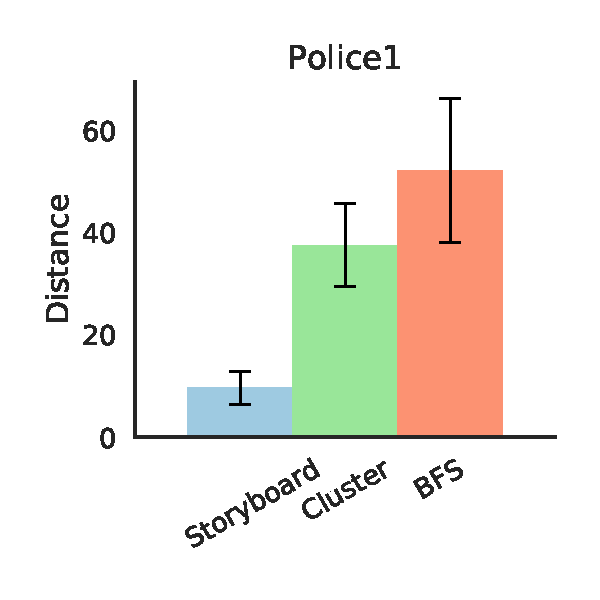
\includegraphics[scale=0.4]{figures/Police1.pdf}
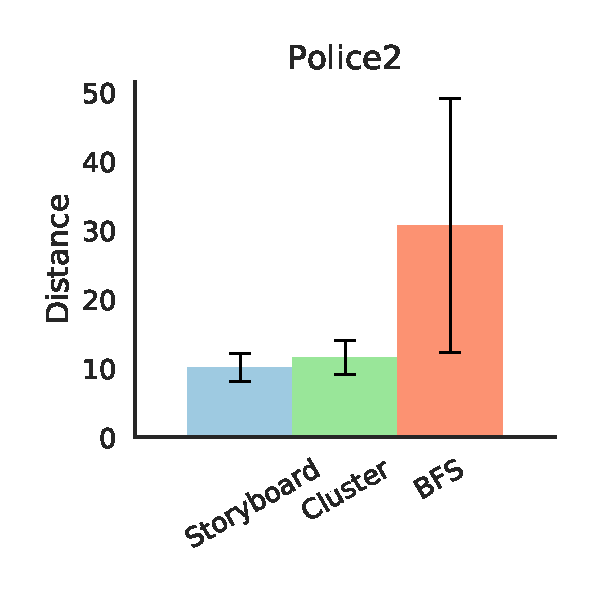
\includegraphics[scale=0.4]{figures/Police2.pdf}
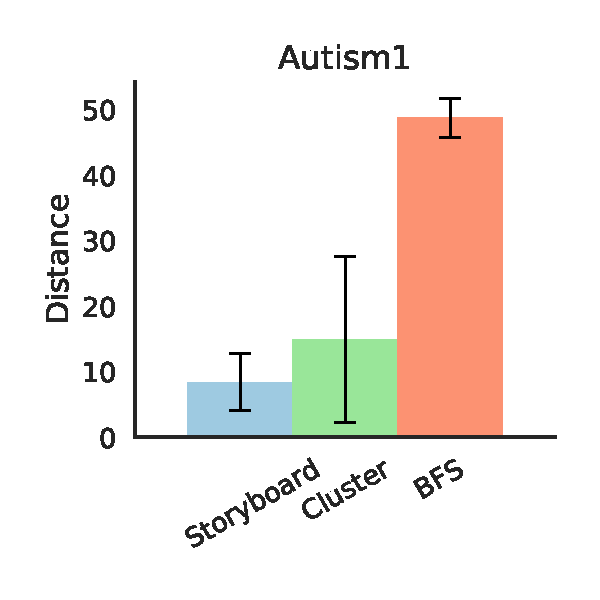
\includegraphics[scale=0.4]{figures/Autism1.pdf}
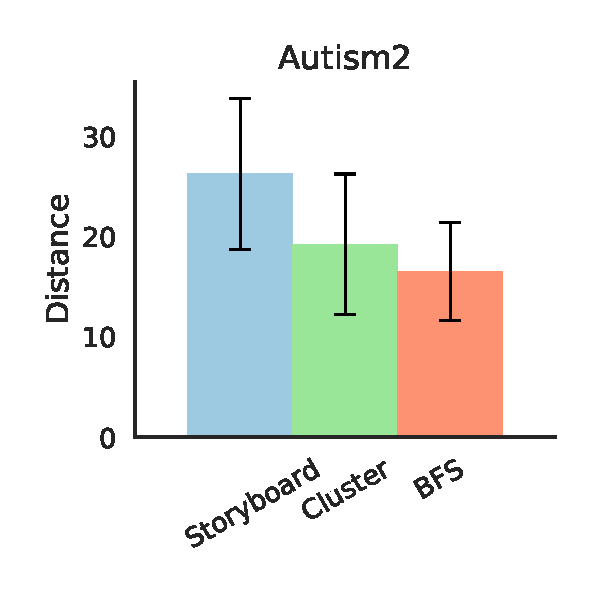
\includegraphics[scale=0.4]{figures/Autism2.pdf}
\caption{Euclidean distance between predicted and ground truth.}
\end{figure}
\subsection{Qualitative results}
through an open coding process by two of the authors.